% Week 4 Explain / Defend receipt -- student starter template.
%
% This is a STARTING SCAFFOLD, not a finished handout. Fill in every
% [FILL IN] marker, delete the italic hand-holding prompts once you've
% used them, and delete this comment block before you submit.
%
% Build it the same way the course builds everything else:
%   latexmk -pdf -interaction=nonstopmode -halt-on-error -outdir=build \
%     explain_defend_receipt.tex
%
% This matches the six-field structure from Wednesday's lesson and the
% Week 04 - Architecture Investigation assignment on Canvas. Choose ONE
% bounded machine claim -- do not try to explain the whole computer.

\documentclass[11pt]{article}
\usepackage[margin=1in]{geometry}
\usepackage{graphicx}
\usepackage{hyperref}
\usepackage{listings}
\usepackage{xcolor}
\usepackage{tcolorbox}
\usepackage{tikz}
\usetikzlibrary{positioning,fit,backgrounds,arrows.meta}

\lstset{
  basicstyle=\ttfamily\small,
  columns=fullflexible,
  keepspaces=true,
  showstringspaces=false,
  breaklines=true,
  frame=single,
}

\tcbset{
  colframe=black!60,
  colback=black!3,
  boxrule=0.6pt,
  arc=1mm,
  fonttitle=\bfseries,
}

\title{Explain / Defend Receipt: Week 4}
\author{[FILL IN: your name]}
\date{\today}

\begin{document}
\maketitle

\section*{Question}
% What vague thing did you want to know about the machine? Narrow it to
% ONE observable subquestion -- "what is this computer doing?" is too
% big; "how many logical processors are visible to my shell right now?"
% is the right size.
[FILL IN: the one bounded question you chose]

\section*{Instrument}
% Which command produced your evidence? Show the exact command you ran.
\begin{lstlisting}
[FILL IN: the exact command, e.g. lscpu]
\end{lstlisting}

\section*{Observation}
% Paste ONLY the lines of output that actually matter. Do not paste an
% entire screen of output and expect the reader to find the evidence
% for you -- picking the relevant lines is part of the argument.
\begin{lstlisting}
[FILL IN: the specific output you are relying on]
\end{lstlisting}

\section*{Interpretation}
% What does that observation actually support? Say it as a claim you
% could defend if someone pushed back on it.
[FILL IN: what the observation supports]

\section*{Boundary}
% This is the part students skip and shouldn't. Name ONE concrete thing
% this observation does NOT establish. "It might not be true for other
% systems" is too vague -- be specific about the layer or scope.
\begin{tcolorbox}[title=What this evidence does \emph{not} prove]
[FILL IN: the specific limitation -- e.g. "this describes the container's
visible interface, not the physical host underneath it"]
\end{tcolorbox}

\section*{Revision}
% If you asked this question again, more precisely, what would you ask
% instead -- or what additional instrument would you add?
[FILL IN: how you'd sharpen the question next time]

\clearpage
\section*{Optional visual: evidence scope diagram}
% A "fun tool" for making your Boundary section concrete instead of
% abstract: draw the layers your observation actually passed through,
% and mark which layer your claim is really about. Edit the labels
% below to match YOUR argument -- delete this section if you don't
% want to use it, it is optional enrichment, not a requirement.
%
% The example below shows the shape for a container-based observation
% (e.g. running the course's optional Architecture Telescope image);
% adapt the outer/middle/inner labels for your own setup (bare metal,
% VM, WSL, cloud instance, etc.).

\begin{center}
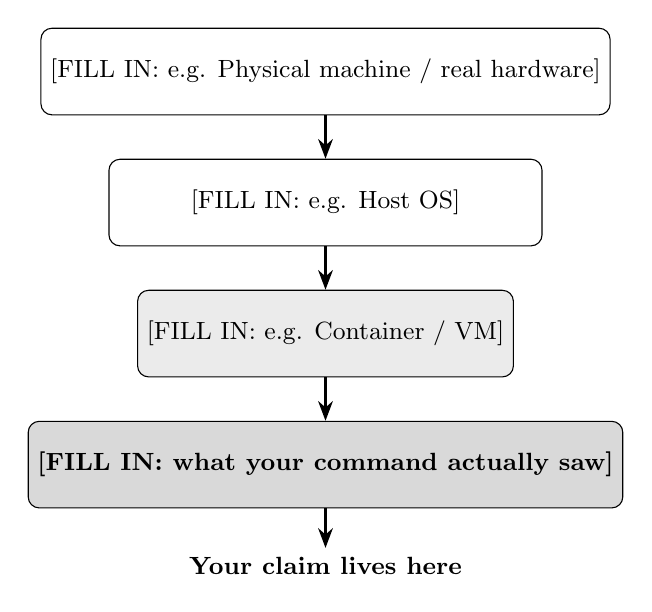
\begin{tikzpicture}[
  layer/.style={draw, rounded corners, minimum width=7cm, minimum height=1.1cm, align=center, font=\small},
  arr/.style={-{Stealth[length=2.5mm]}, thick},
  node distance=0.55cm,
]
  \node[layer] (physical)
    {[FILL IN: e.g. Physical machine / real hardware]};
  \node[layer, below=of physical, minimum width=5.5cm] (host)
    {[FILL IN: e.g. Host OS]};
  \node[layer, below=of host, minimum width=4cm, fill=black!8] (mid)
    {[FILL IN: e.g. Container / VM]};
  \node[layer, below=of mid, minimum width=5cm, fill=black!15] (obs)
    {\textbf{[FILL IN: what your command actually saw]}};

  \draw[arr] (physical) -- (host);
  \draw[arr] (host) -- (mid);
  \draw[arr] (mid) -- (obs);

  \node[below=0.5cm of obs, font=\small\bfseries] (claim) {Your claim lives here};
  \draw[arr] (obs) -- (claim);
\end{tikzpicture}
\end{center}

\emph{Narrower boxes are closer to what your instrument could actually
see; the boxes above it are real, but your evidence says nothing
specific about them.}

\emph{Caption: [FILL IN: one sentence naming exactly which layer your
Instrument actually queried, and which layers it says nothing about.]}

\end{document}
